\section{Introduction}

% [背景：LLM 部署挑战与 MXFP4 的崛起]
% 随着大规模语言模型（LLMs）在各个领域的广泛应用~\cite{qwen3, llama3}，其巨大的参数量和推理时的显存带宽需求已成为实际部署的主要瓶颈~\cite{outliers}。为了在资源受限的边缘设备或大规模数据中心高效运行 LLM，训练后量化（PTQ）已成为业界标准范式~\cite{quik,rsavq,rwkvquant,mquant,moequant}。尽管传统的 INT4 量化在权重压缩上取得了显著成效，但其受限的动态范围难以适配 Transformer 激活中普遍存在的长尾异常值（Outliers） ~\cite{outliers}。鉴于此，工业界正通过硬件协同设计转向具有更高动态范围的低精度浮点格式。其中，开放计算项目（OCP）推出的 MXFP4 (e2m1) 标准，通过引入块级共享指数（Block-wise Shared Exponent）技术，在保持 4-bit 压缩率的同时提供了接近 FP8 的表示能力，并已获得 NVIDIA Blackwell 和 AMD Ryzen AI 等下一代硬件的原生支持 ~\cite{ostquant,singlequant}。MXFP4 被广泛视为下一代低比特推理的基石。
With the widespread adoption of Large Language Models (LLMs) across various domains~\cite{qwen3, llama3}, their massive parameter counts and the memory bandwidth demanded during inference have become major bottlenecks for practical deployment~\cite{outliers}. To run LLMs efficiently on resource-constrained edge devices or in large-scale data centers, Post-Training Quantization (PTQ) has emerged as the industry standard paradigm~\cite{quik,rsavq,rwkvquant,mquant,moequant}. While traditional INT4 quantization has achieved significant success in weight compression, its limited dynamic range struggles to accommodate the long-tail outliers prevalent in Transformer activations~\cite{outliers}. Consequently, the industry is shifting toward low-precision floating-point formats with higher dynamic ranges through hardware co-design. Notably, the MXFP4 (e2m1) standard introduced by the Open Compute Project (OCP), which employs Block-wise Shared Exponent technology, offers representation capabilities approaching FP8 while maintaining 4-bit compression rates. Supported natively by next-generation hardware such as NVIDIA Blackwell and AMD Ryzen AI~\cite{ostquant,singlequant}, MXFP4 is widely regarded as the cornerstone of next-generation low-bit inference.

% 【挑战：MXFP4 激活量化的“水土不服”】
% 然而，尽管 MXFP4 理论优势明显，我们的实证分析表明，直接将其应用于 LLM 激活量化会面临严峻的精度瓶颈。现有的先进量化方法，如SingleQuant~\cite{singlequant}、DARTQuant~\cite{dartquant}、FlatQuant~\cite{flatquant}与OSTQuant~\cite{ostquant}，虽然通过旋转技术成功解决了 W4A4 整数量化问题，但它们主要是为了抑制异常值以适配整数的均匀网格 。这种设计忽视了 MXFP4 独特的块浮点（Block Floating Point）拓扑结构。简单地将针对整数优化的旋转策略迁移到 MXFP4 上，往往无法发挥浮点格式的潜力，甚至适得其反。
\begin{figure}[htbp] 
    \centering  
    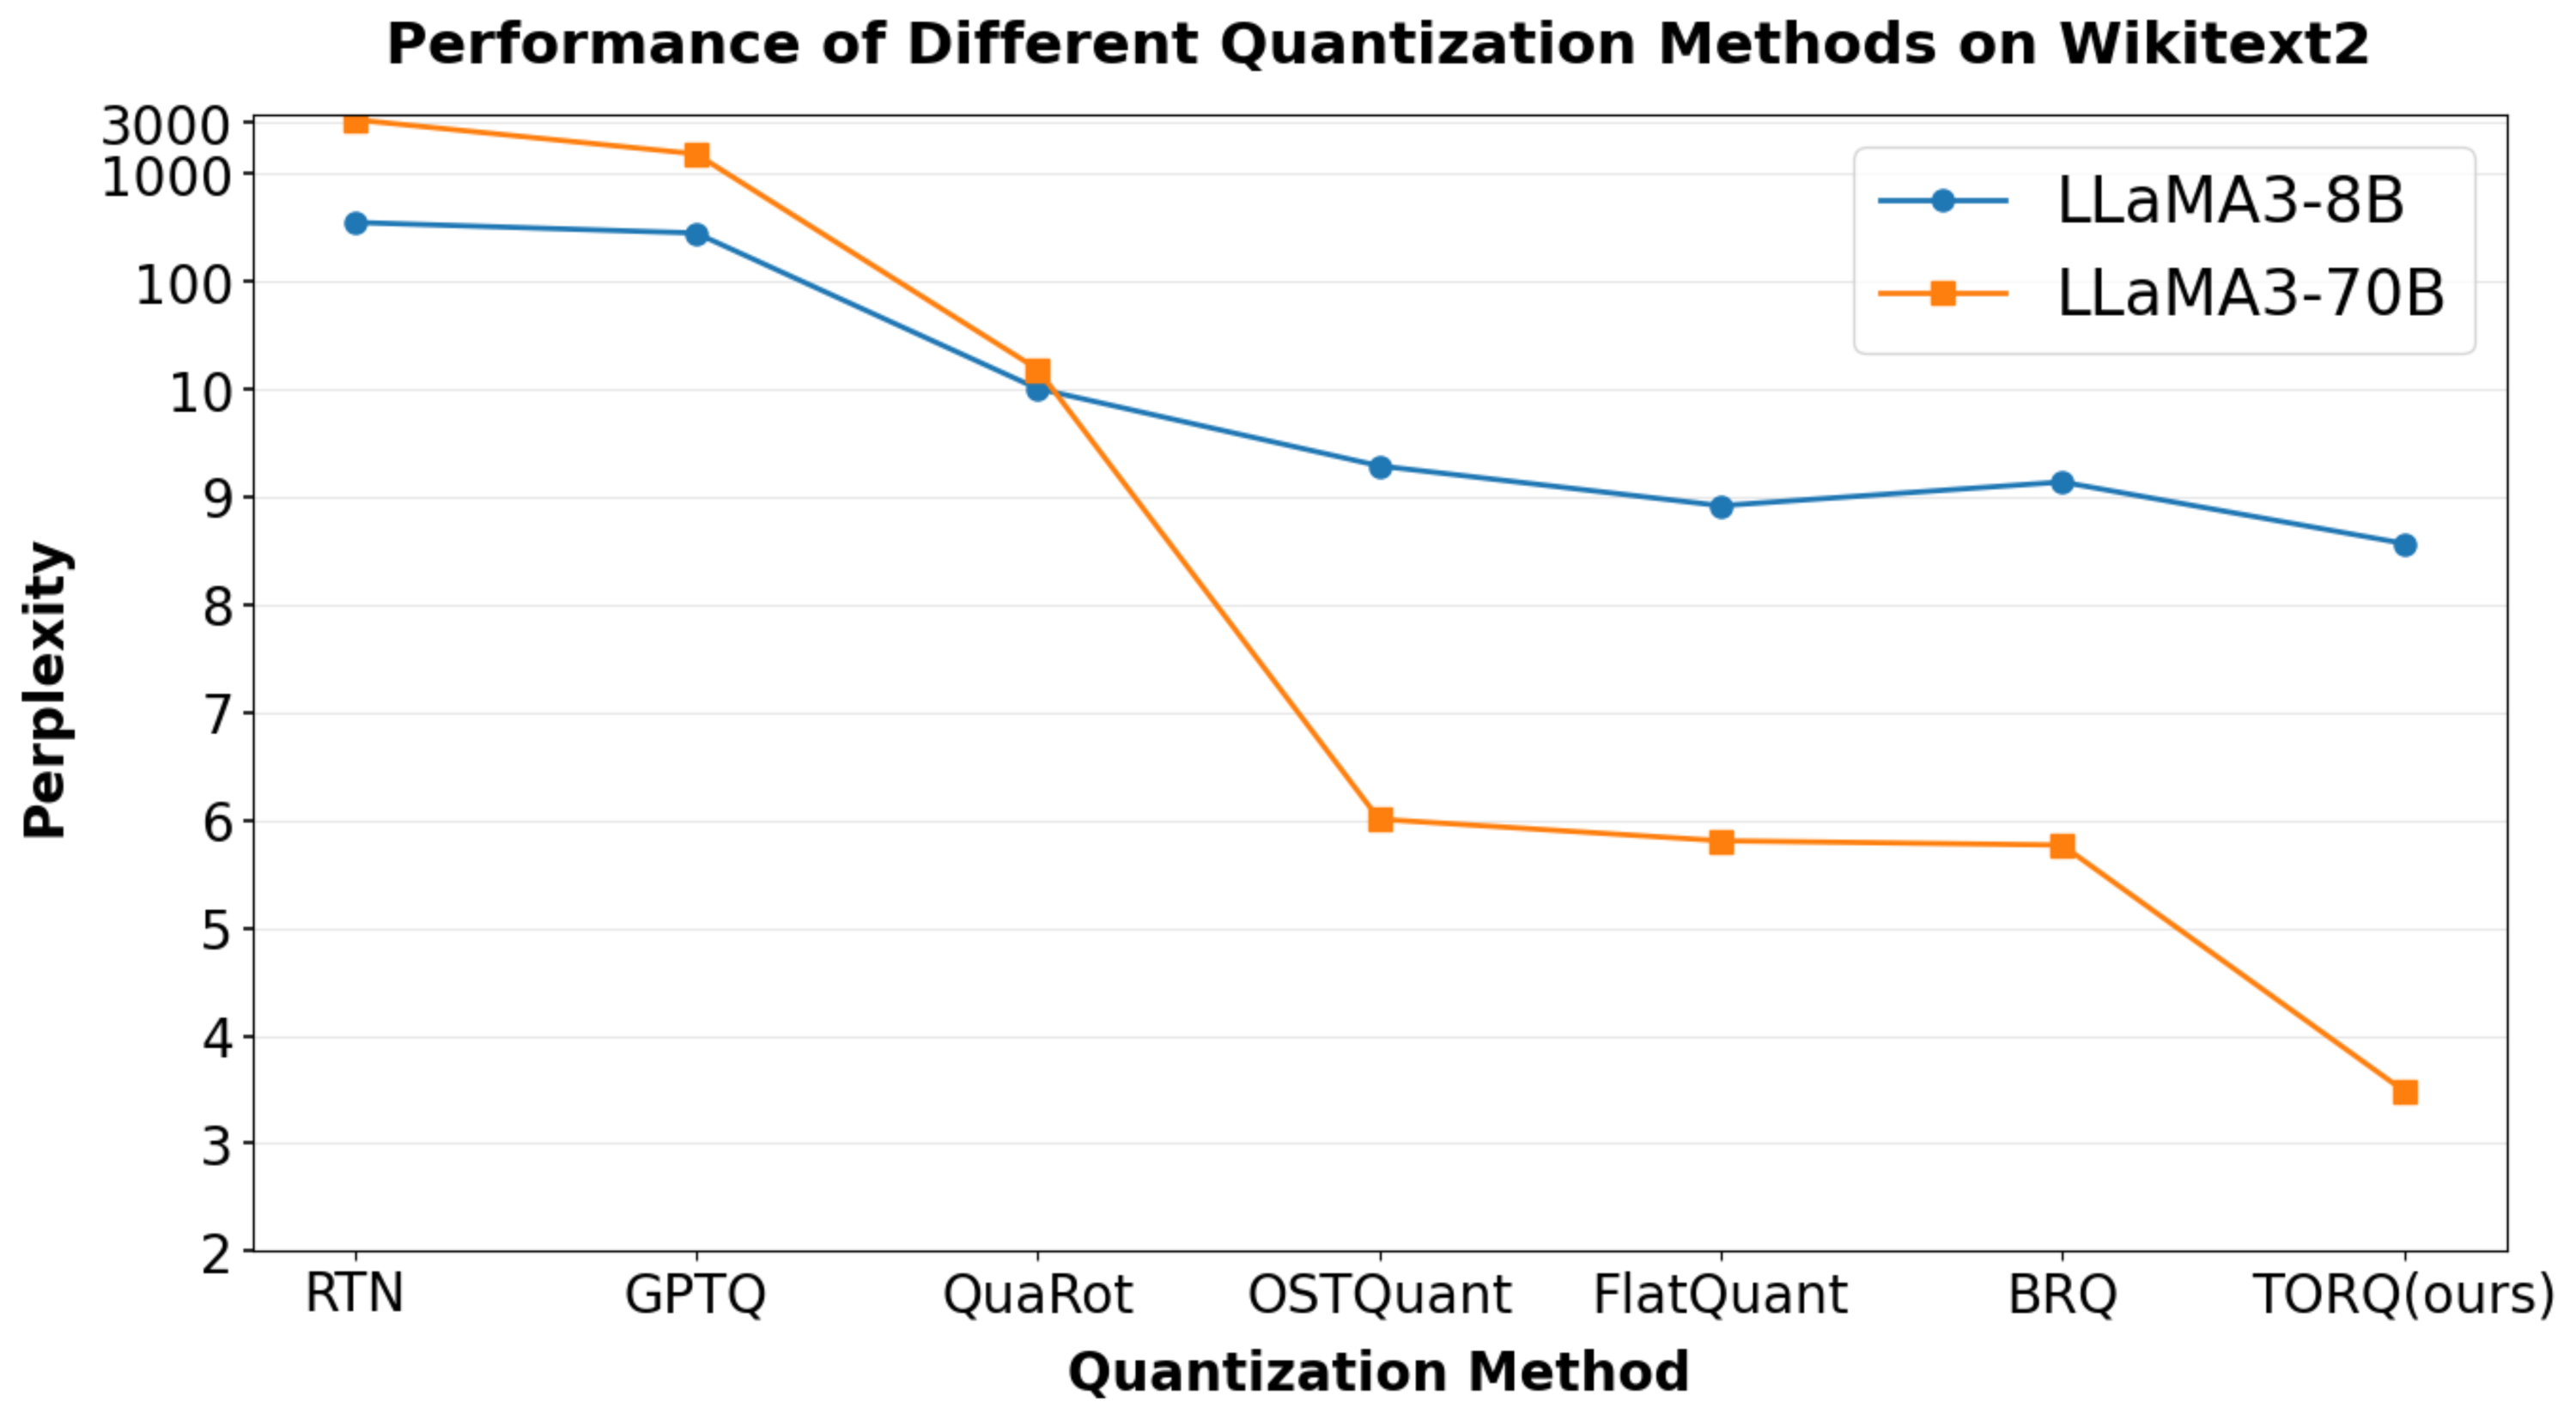
\includegraphics[width=0.45\textwidth]{img/fig_intro_ppl.png}
    \caption{Performance of Different Quantization Methods on LLaMA3-8B and LLaMA3-70B.}
    \label{fig:quantization_performance}
\end{figure}
% \vspace{-4mm}
Despite the theoretical advantages of MXFP4, our empirical analysis reveals that directly applying it to LLM activation quantization encounters severe accuracy bottlenecks. State-of-the-art quantization methods, such as SingleQuant~\cite{singlequant}, DARTQuant~\cite{dartquant}, FlatQuant~\cite{flatquant}, and OSTQuant~\cite{ostquant}, have successfully addressed W4A4 integer quantization through rotation techniques. However, these methods are primarily designed to suppress outliers to fit the uniform grid of integers. This design overlooks the unique Block Floating Point (BFP) topological structure of MXFP4. As a result, simply transferring rotation strategies optimized for integers to MXFP4 often fails to exploit the potential of the floating-point format and may even be counterproductive.

% 【洞察：阻碍精度的两大结构性失衡--motivation】
% 为了解开这一难题，本文深入剖析了 MXFP4 激活量化的误差结构，揭示了导致精度下降的根本原因在于激活分布与 MXFP4 格式之间存在的两大结构性挑战：1.跨块方差极度不均衡 (Inter-block Variance Imbalance)。MXFP4 的量化精度高度依赖于块内共享指数（Scaling Factor）。当激活向量被切分为固定块（如 Block Size=32）时，块方差呈现显著的重尾分布。少数高能量块不仅主导了总均方误差（MSE），更迫使共享指数剧烈抬升，导致同块内 90% 以上的中小幅值元素由于分辨率不足而归零。2.块内码本利用不均衡 (Intra-block Codebook Collapse)。MXFP4 的 e2m1 码本设计假设数据服从理想的对数正态分布。然而，真实激活分布往往高度集中于零点附近，导致绝大多数数值落在最小量化间隔内，而大量表示能力较强的大值码字处于闲置状态（即 Codebook Collapse）。我们的统计显示，如图2所示，约 50% 的码字区间在实际推理中仅被10%数据激活，造成了严重的比特浪费。
\begin{figure*}[ht!] 
    \centering  
    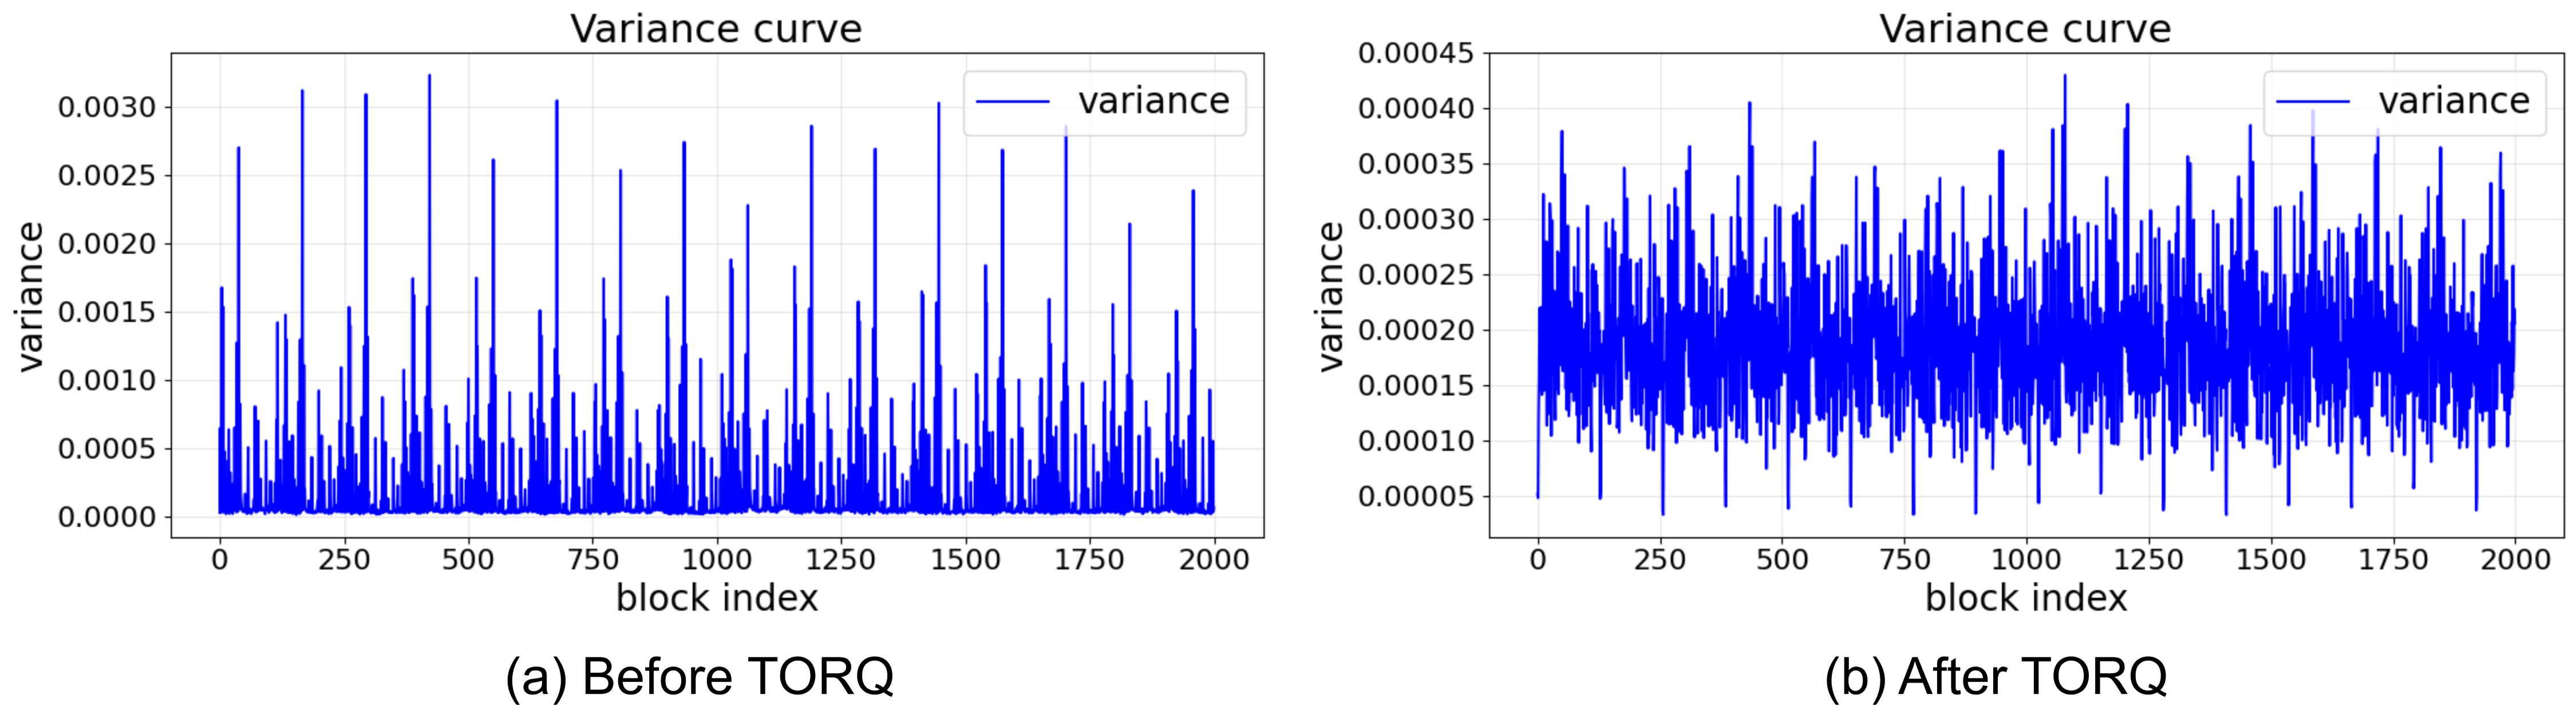
\includegraphics[width=0.95\textwidth]{img/fig-motivation_1.png}
    \caption{MXFP4 Quantization of each micro block's variance distribution: (a) Variance distribution of original data without TORQ, (b) Variance distribution after TORQ processing}
    \label{fig:motivation_1}
\end{figure*}
To address this challenge, this paper conducts an in-depth analysis of the error structure of MXFP4 activation quantization, revealing that the root cause of accuracy degradation lies in two structural conflicts between the activation distribution and the MXFP4 format: (1).Extreme Inter-block Variance Imbalance: The quantization accuracy of MXFP4 relies heavily on the block-wise shared scaling factor. When the activation vector is partitioned into fixed blocks (e.g., Block Size=32), as shown in Figure.\ref{fig:motivation_1}, block variance exhibits a significant heavy-tailed distribution. A minority of high-energy blocks not only dominate the total Mean Squared Error (MSE) but also force the shared exponent to rise sharply, causing over 90\% of small-magnitude elements within the same block to be zeroed out due to insufficient resolution. 
% 【Therefore, our 'Variance Equalization' is not an end in itself, but a mathematically optimal strategy to minimize the maximum required shared exponent across blocks, thereby preserving the precision of non-outlier elements.】
(2).Intra-block Codebook Utilization Imbalance (Codebook Collapse): The e2m1 codebook design of MXFP4 assumes data follows an ideal log-normal distribution. However, real-world activation distributions are often highly concentrated near zero, causing the vast majority of values to fall within the minimum quantization interval, while numerous codewords with strong representation capabilities for large values remain idle (i.e., Codebook Collapse). As shown in Figure.\ref{fig:motivation_2}, our statistics show that approximately 50\% of the codeword range is activated by only 10\% of the data in actual inference, resulting in severe bit waste.
\begin{figure*}[h] 
    \centering  
    
\includegraphics[width=0.95\textwidth]{img/fig-motivation_2.png}
    \caption{Histogram statistics of each codeword quantified by FP4(e2m1):(a) Codeword occupancy of the original data without TORQ, (b) Codeword occupancy after TORQ processing}
    \label{fig:motivation_2}
\end{figure*}

% 【提出我们的方法】
% 基于上述关键洞察，我们提出 TORQ(Two-level Orthogonal Rotation for MXFP4 Quantization) 。这是一种无需重训练的 PTQ 框架，其核心理念是：与其被动调整量化参数以适应病态的激活分布，不如主动旋转激活坐标系，使其分布特性与 MXFP4 的结构特性对齐。TORQ 将优化问题解耦为两个数学上正交的子问题：1.宏观均衡旋转 (Macro-Equilibrium Rotation)：针对跨块方差不均衡，TORQ 基于 Schur-Horn 定理，构造块间正交变换将激活能量在所有块之间均匀“摊平”。我们从理论上证明了，这种方差全均衡配置是最小化全局量化误差的最优解。2.微观对齐旋转(Micro-Alignment Rotation)：针对块内码本利用率低，TORQ 引入最大熵原理，在组内执行正交旋转，重塑局部数据分布，使其在 FP4 空间中均匀“流入”各个码字区间，从而最大化有效信息容量。
Based on these key insights, we propose TORQ (Two-level Orthogonal Rotation for MXFP4 Quantization). This is a retraining-free PTQ framework whose core philosophy is: Instead of passively adjusting quantization parameters to fit ill-conditioned activation distributions, we should actively rotate the activation coordinate system to align its distribution characteristics with the structural properties of MXFP4. 
TORQ decouples the optimization problem into two mathematically orthogonal sub-problems: 
(1).Macro-Equilibrium Rotation: To address inter-block variance imbalance, TORQ constructs an inter-block orthogonal transformation based on the Schur-Horn theorem to uniformly distribute activation energy across all blocks. We theoretically prove that this variance-equalized configuration is the optimal solution for minimizing global quantization error. (2).Micro-Alignment Rotation: To address low intra-block codebook utilization, TORQ introduces the principle of maximum entropy to execute orthogonal rotation within groups. This reshapes the local data distribution to "flow" uniformly into each codeword interval in the FP4 space, thereby maximizing effective information capacity.

% 【我们方法的结果】
% TORQ 仅需少量校准数据即可闭式构造旋转矩阵，且在推理阶段引入的旋转矩阵参数规模极小，几乎不会产生额外计算开销。在 LLaMA、Qwen 等主流大语言模型（LLM）上的实验结果表明，TORQ 的性能显著优于当前的最优方法（SOTA）。如图 3 所示，在 Llama3 系列模型中，该方法的表现始终超越现有的先进量化方案。以 Qwen3-8B 模型为例：在 WikiText 数据集上，其困惑度仅为 10.26，相较浮点模型仅提升 1.26；平均准确率则从 30.73% 大幅提升至 67.75%，较 FlatQuant 方法领先 1.79 个百分点，成功解决了 4-bit 浮点量化场景下的精度下降难题。
% 本文贡献：
%   - 首次系统性地识别并形式化了阻碍 MXFP4 性能的两大结构性挑战——跨块方差不均衡与块内码本利用不均衡 。
%   - 出了首个针对块浮点结构设计的双级旋转框架 TORQ，通过宏观方差均衡与微观码本对齐，实现了量化误差的系统性最小化 。
%   - 为两级旋转建立了坚实的理论基础。证明了在凸误差模型下，方差均衡配置近似最优；同时，论证了在MXFP4几何结构下，码字占用均衡近似于最小化量化误差。
%   - 设计了无需微调的PTQ流程，在多种LLM和多样化的下游任务上验证了方法的有效性、普适性及硬件友好性。

TORQ enables the closed-form construction of rotation matrices using only a minimal volume of calibration data. Furthermore, the rotation matrices incorporated during the inference phase feature an extremely compact parameter footprint, imposing negligible additional computational overhead.Experimental evaluations on mainstream large language models (LLMs), including LLaMA and Qwen, demonstrate that TORQ achieves a significant performance superiority over prevailing state-of-the-art (SOTA) approaches. As illustrated in Figure.\ref{fig:quantization_performance}, this method consistently outperforms existing advanced quantization schemes across the entire Llama3 model series. Taking the Qwen3-8B model as a representative case: on the WikiText dataset, it attains a perplexity score of merely 10.26, representing a marginal increase of 1.26 compared with the full-precision floating-point baseline. Meanwhile, its average accuracy is boosted substantially from 30.73\% to 67.75\%, outperforming the FlatQuant method by a margin of 1.79 percentage points. Collectively, these results confirm that TORQ effectively mitigates the accuracy degradation challenge inherent to 4-bit floating-point quantization scenarios.
Our Contributions:
\begin{itemize}
    \item We systematically identify and formalize, for the first time, the two structural challenges hindering MXFP4 performance: Inter-block Variance Imbalance and Intra-block Codebook Utilization Imbalance.
    \item We propose TORQ, the first dual-level rotation framework explicitly designed for block floating-point structures. By integrating macro-variance equilibrium and micro-codebook alignment, it achieves a systematic minimization of quantization error.
    \item We establish a solid theoretical foundation for two-level rotation. We prove that under a convex error model, the variance equilibrium configuration is approximately optimal; meanwhile, we demonstrate that under the MXFP4 geometric structure, codeword occupancy equilibrium approximates the minimization of quantization error.
    \item We design a fine-tuning-free PTQ pipeline and verify the method's effectiveness, universality, and hardware friendliness across multiple LLMs and diverse downstream tasks.
\end{itemize}